\subsection{Base radiale (RBF)}
\newcommand{\factnorm}{\sum_{r=1}^{m}x_{r}}
\subsubsection{Neurone}
Un neurone \textbf{caché} d'un \rbf n'effectue pas de somme pondérée de ses entrées.
Il applique directement sa fonction d'activation $\phi$, une gaussienne de moyenne $\mu$ et d'écart-type $\sigma$ où $x$, de dimension $n$, est l'entrée du neurone.
\begin{equation}\label{eq:cachephi}
 \phi(x) = e^{-\frac{1}{2}\sum_{k=1}^{n}\frac{(x_k-\mu_{ik})^2}{\sigma_{ik}^{2}}}
\end{equation}
Où $i$ est l'indice du neurone. $\mu$ s'appelle aussi \emph{prototype} dans le cas d'un \rbf.
%$\phi(x)$ peut se résumer en: \[\phi(x) = e^{-\beta||x-\mu||^2}\]Où $\beta$ est donc un coefficient qui règle la largeur de la courbe en cloche.\\
\\

Un neurone \textbf{de sortie} d'un \rbf n'effectue pas non plus de somme pondérée de ses entrées. Sa fonction d'activation est:
\begin{equation}\label{eq:sortiephi}
 \phi(x) = \frac{\sum_{j=1}^{m}W_{ij}x_{j}}{\sum_{j=1}^{m}x_{j}}
\end{equation}
Où $i$ est l'indice du neurone et $x$ l'entrée de dimension $m$.
\begin{figure}
 \centering
 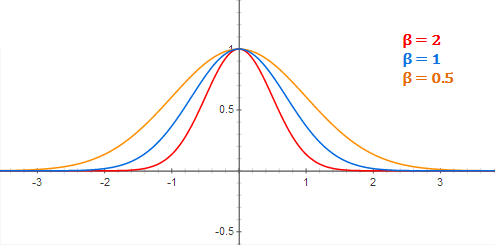
\includegraphics[scale=0.7]{../figures/RBFactivation.png}
 \caption{Activation d'un neurone RBF avec différentes valeurs d'écart-type}
 \label{rbfactivation}
\end{figure}
La Figure \ref{rbfactivation} représente la sortie d'un neurone \rbf où $\mu$ et $x$ sont de dimension 1 et $\mu = 0$.\\
Pour résumer, un neurone \rbf renvoie une valeur indiquant la simularité entre l'entrée et son prototype.
\subsubsection{Structure}
\begin{figure}
 \centering
 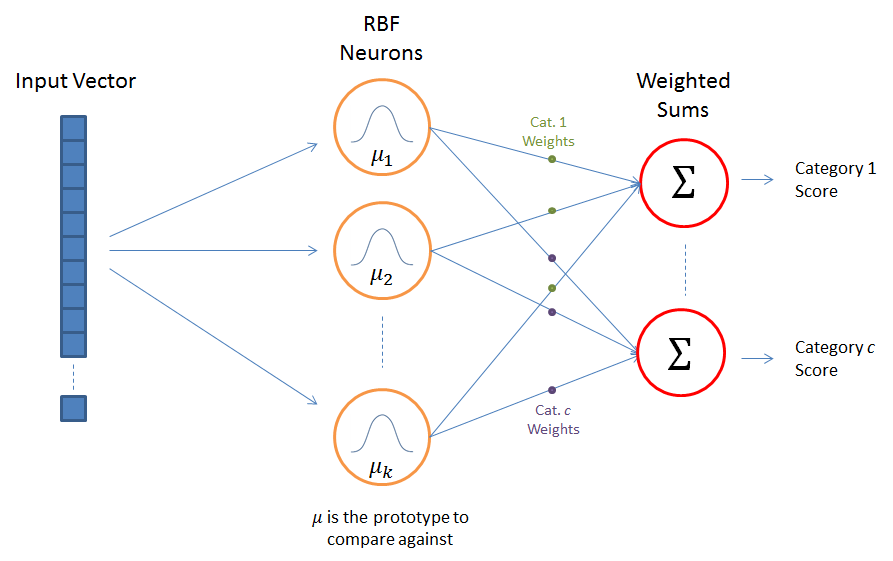
\includegraphics[scale=0.5]{../figures/RBFstruct.png}
 \caption{Structure RBF. \textbf{Source}: McCormick\cite{RBFtuto}}
 \label{structurerbf}
\end{figure}
La structure d'un \rbf est comme celle du \mlp sauf qu'il n'y a qu'une seule couche cachée (Figure \ref{structurerbf}).
\subsubsection{Apprentissage}
Dans ce réseau, les paramètres qui seront modifiés lors de l'apprentissage sont les poids des neurones de sortie et les moyennes et écart-types des neurones cachés.
L'algorithme de rétropropagation peut être utilisé pour un apprentissage supervisé d'un \rbf.
Reprenons \eqref{eq:Q}, l'erreur quadratique $Q$ défini dans la section \ref{sec:appmlp}.
En reprenant le même raisonnement que la rétropropagation dans un \mlp,
on va faire un pas de $\eta$ dans le sens opposé et proportionnel au gradient pour chaque poid $W_{ij}$ des neurones de sortie mais aussi des prototypes $\mu_i$ et écart-types $\sigma_i$ des neurones cachés.
C'est à dire que les paramètres seront modifiés de la sorte:
\begin{equation}\label{eq:modifpoid}
 \Delta W_{ij} = -\eta \partiel{Q}{W_{ij}}
\end{equation}
\begin{equation}\label{eq:modifmu}
 \Delta \mu_{ik} = -\eta \partiel{Q}{\mu_{ik}}
\end{equation}
\begin{equation}\label{eq:modifsigma}
 \Delta \sigma_{ik} = \eta \partiel{Q}{\sigma_{ik}}
\end{equation}

D'abord déterminons le facteur $\partiel{Q}{W_{ij}}$ dans \eqref{eq:modifpoid}. On est dans le cas où $i$ est un neurone de sortie.
Par \eqref{eq:Q}, $Q$ dépend de $\phi_i$. Par \eqref{eq:sortiephi}, $phi_i$ dépend de $W_{ij}$.
Par le théorème de dérivée des fonctions composés,
\begin{equation}\label{eq:rbfsortie}
 \partiel{Q}{W_{ij}} = \partiel{Q}{\phi_i} \partiel{\phi_i}{W_{ij}}
\end{equation}
Par \eqref{eq:sortie1}, on sait que
\[\partiel{Q}{\phi_i} = (\phi_i - s_i)\]
Ensuite,
\begin{equation}\label{eq:poidgrad}
 \begin{split}
  \partiel{\phi_i}{W_{ij}} & = \partiel{\frac{\sum_{r=1}^{m}W_{ir}x_{j}}{\factnorm}}{W_{ij}}\\
  ~ & = \frac{1}{\factnorm} \partiel{\sum_{r=1}^{m}W_{ir}x_{j}}{W_{ij}}\\
  ~ & = \frac{1}{\factnorm} \partiel{\left(W_{i1}x_1 + W_{i2}x_2 + ... + W_{ij}x_j + ... + W_{im}x_m\right)}{W_{ij}}\\
  ~ & = \frac{1}{\factnorm} \left(\partiel{W_{i1}x_1}{W_{ij}} + \partiel{W_{i2}x_2}{W_{ij}} + ... + \partiel{W_{ij}x_j}{W_{ij}} + ... + \partiel{W_{im}x_m}{W_{ij}}\right)\\
  ~ & = \frac{1}{\factnorm} \left(0 + 0 + ... + x_j + ... + 0\right)\\
  ~ & = \frac{x_j}{\factnorm}
 \end{split}
\end{equation}
Subsituons \eqref{eq:sortie1} et \eqref{eq:poidgrad} dans \eqref{eq:rbfsortie}.
\begin{equation}\label{eq:sortiegrad}
 \partiel{Q}{W_{ij}} = (\phi_i - s_i) \frac{x_j}{\factnorm}
\end{equation}
Et \eqref{eq:sortiegrad} dans \eqref{eq:modifpoid},
\[\Delta W_{ij} = -\eta (\phi_i - s_i) \frac{x_j}{\factnorm}\]\\

Déterminons maintenant le facteur $\partiel{Q}{\mu_{ik}}$ dans \eqref{eq:modifmu}. On est dans le cas où $i$ est un neurone caché.
$Q$ dépend de $\phi_i$ qui lui-même est fonction de $\mu_{ik}$. Par le théorème de dérivée de fonction composés,
\begin{equation}\label{eq:composemu}
 \partiel{Q}{\mu_{ik}} = \partiel{Q}{\phi_i} \partiel{\phi_i}{\mu_{ik}}
\end{equation}
On va déterminer la valeur de $\partiel{Q}{\phi_i}$ et puis de $\partiel{\phi_i}{\mu_{ik}}$.
Soit $j$ un neurone de sortie. On sait que $Q$ dépend de tous les $\phi_j$ et les $\phi_j$ dépendent de $\phi_i$. On sait donc que
\begin{equation}\label{eq:mufact1}
 \partiel{Q}{\phi_i} = \sum_{j} \partiel{Q}{\phi_j}\partiel{\phi_j}{\phi_i}
\end{equation}
Par \eqref{eq:sortie1}, on sait que
\[\partiel{Q}{\phi_j} = (\phi_j - s_j)\]
Et posons $x_r$ l'entrée de $j$ provenant de $i$, c'est à dire $\phi_i = x_r$.
Posons $n$ la dimension de l'entrée de $j$.
Posons aussi $R = \sum_{k=1}^{n}x_k$.
Pour trouver la valeur de $\partiel{\phi_j}{\phi_i}$, nous aurons besoin de trouver $\partiel{\frac{1}{R}}{x_k}$.
\begin{equation}\label{eq:1sr}
 \begin{split}
 \partiel{\frac{1}{R}}{x_k} & = \frac{-1}{R^2}\partiel{R}{x_k}\\
 ~ & = \frac{-1}{R^2}\partiel{x_1+x_2+...+x_k+...+x_n}{x_k}\\
 ~ & = \frac{-1}{R^2} 1
 \end{split}
\end{equation}
Dès lors, utilisons \eqref{eq:1sr} pour simplifier l'équation suivante;
\begin{equation}\label{eq:phiiphij}
 \begin{split}
 \partiel{\phi_j}{\phi_i} & = \partiel{\phi_j}{x_r}\\
 ~ & = \partiel{\left(\frac{\sum_{k=1}^{n}W_{jk}x_k}{\sum_{k=1}{n}x_k}\right)}{x_r}\\
 ~ & = \partiel{\left(\frac{W_{j1}x_1}{R} + \frac{W_{j2}x_2}{R} + ... + \frac{W_{jr}x_r}{R} + ... + \frac{W_{jn}x_n}{R}\right)}{x_r}\\
 ~ & = \partiel{\left(\frac{W_{j1}x_1}{R}\right)}{x_r} + \partiel{\left(\frac{W_{j2}x_2}{R}\right)}{x_r} + ... + \partiel{\left(\frac{W_{jr}x_r}{R}\right)}{x_r} + .. + \partiel{\left(\frac{W_{jn}x_n}{R}\right)}{x_r}\\
 ~ & = (W_{j1}x_1)\frac{-1}{R^2} + (W_{j2}x_2)\frac{-1}{R^2} + ... + \left[(W_{jr}x_r)\partiel{\frac{1}{R}}{x_r}+\partiel{(W_{jr}x_r)}{x_r}\frac{1}{R}\right] + ... + (W_{jn}x_n)\frac{-1}{R^2}\\
 ~ & = (W_{j1}x_1)\frac{-1}{R^2} + (W_{j2}x_2)\frac{-1}{R^2} + ... + \left[(W_{jr}x_r)\frac{-1}{R^2}+W_{jr}\frac{1}{R}\right] + ... + (W_{jn}x_n)\frac{-1}{R^2}\\
 ~ & = \left(\sum_{k=1}^{n}W_{jk}x_k\frac{-1}{R^2}\right)-W_{jr}x_r\frac{-1}{R^2} + \left[(W_{jr}x_r)\frac{-1}{R^2}+W_{jr}\frac{1}{R}\right]\\
 ~ & = \frac{-1}{R^2} \left[\left(\sum_{k=1}^{n}W_{jk}x_k\right)-W_{jr}x_r + (W_{jr}x_r) + W_{jr}(-R)\right]\\
 ~ & = \frac{-1}{R^2} \left(W_{jr}(-R) + \sum_{k=1}^{n}W_{jk}x_k\right)\\
 ~ & = \frac{1}{R^2} \left(W_{jr}R - \sum_{k=1}^{n}W_{jk}x_k\right)
 \end{split}
\end{equation}
On substitue \eqref{eq:sortie1} et \eqref{eq:phiiphij} dans \eqref{eq:mufact1} pour obtenir
\begin{equation}\label{eq:mufacto1}
 \partiel{Q}{\phi_i} = \sum_{j} (\phi_j - s_j) \frac{1}{R^2} \left(W_{jr}R - \sum_{k=1}^{n}W_{jk}x_k\right)
\end{equation}

Si nous calculons $\partiel{\phi_i}{\mu_{ik}}$, nous obtenons
\begin{equation}\label{eq:mufacto2}
 \partiel{\phi_i}{\mu_{ik}} = \phi_i \frac{x_k-\mu_{ik}}{\sigma_{ik}^2}
\end{equation}
Et en substituant \eqref{eq:mufacto1} et \eqref{eq:mufacto2} dans \eqref{eq:composemu},
\[\partiel{Q}{\mu_{ik}} = \left[\sum_{i}(\phi_j - s_j) \frac{1}{R^2} \left(W_{jr}R - \sum_{k=1}^{n}W_{jk}x_k\right)\right] \phi_i\frac{x_k-\mu_{ik}}{\sigma_{ik}^2}\]
Qu'on substitue dans \eqref{eq:modifmu}, on obtient la modification à appliquer sur $\mu_{ik}$:
\[\Delta\mu_{ik} = -\eta \left[\sum_{i}(\phi_j - s_j) \frac{1}{R^2} \left(W_{jr}R - \sum_{k=1}^{n}W_{jk}x_k\right)\right] \phi_i\frac{x_k-\mu_{ik}}{\sigma_{ik}^2}\]

Enfin déterminons le facteur $\partiel{Q}{\sigma_{ik}}$ dans \eqref{eq:modifsigma}. On est dans le cas où $i$ est un neurone caché.
$Q$ dépend de $\phi_i$ qui lui-même est fonction de $\sigma_{ik}$. Par le théorème de dérivée de fonction composés,
\begin{equation}\label{eq:composesigma}
 \partiel{Q}{\sigma_{ik}} = \partiel{Q}{\phi_i} \partiel{\phi_i}{\sigma_{ik}}
\end{equation}
Si nous calculons $\partiel{\phi_i}{\sigma_{ik}}$, nous obtenons
\begin{equation}\label{eq:sigmafacto2}
 \partiel{\phi}{\sigma_{ik}} = \phi_i \frac{(x_k-\mu_{ik})^2}{\sigma_{ik}^3}
\end{equation}
On peut substituer \eqref{eq:mufacto1} et \eqref{eq:sigmafacto2} dans \eqref{eq:composesigma}:
\[\left[\sum_{i}(\phi_j - s_j) \frac{1}{R^2} \left(W_{jr}R - \sum_{k=1}^{n}W_{jk}x_k\right)\right] \phi_i \frac{(x_k-\mu_{ik})^2}{\sigma_{ik}^3}\]
Qu'on substitue dans \eqref{eq:modifsigma}, on obtient la modification à appliquer sur $\sigma_{ik}$:
\[\Delta \sigma_{ik} = -\eta \left[\sum_{i}(\phi_j - s_j) \frac{1}{R^2} \left(W_{jr}R - \sum_{k=1}^{n}W_{jk}x_k\right)\right] \phi_i \frac{(x_k-\mu_{ik})^2}{\sigma_{ik}^3}\]

\subsubsection{Applications}
Un \rbf peut aussi servir pour la classification non linéaire.\cite{statistica}